\section{Background}

In this section, we provide a brief summary to passivity-based control and the
recent data-driven variant our group has introduced in~\cite{ashenafi2022robust,
sirichotiyakul2022data, acc}.
%
We also motivate the advantages of the Bayesian learning framework in
uncertainty modeling and robust control.
\subsection{Passivity-Based Control (PBC)}
\label{ssec:pbc}

Suppose we have a robotic system whose Hamiltonian $H : \mathcal{X} \rightarrow
\mathbb{R}$ can be expressed as
%
\begin{equation}
    H(q,p) = \frac{1}{2} p^\top M^{-1}(q) p + V(q),
    \label{eq:system_hamiltonian}
\end{equation}
%
where $p \in \mathbb{R}^m$ is the generalized momenta, and $V(q)$ represents the
potential energy. Hamilton's equations of motion are given by
\begin{align}
    \begin{split}  
      f(x, u) &= \bmat{\nabla_pH \\ -\nabla_qH}\ + \bmat{0 \\ \Omega(q)}u, \\
      &\hspace{-0.15cm} y = \Omega(q)^\top \dot{q},
    \end{split}
    \label{eq:hamiltonian_dynamics}
\end{align}
\noindent where $x = (q, p)$, $\Omega(q) \in \mathbb{R}^{m \times n}$ is
the input matrix, and $u \in \mathbb{R}^{n}$ is the control input.
%
% The system~\eqref{eq:hamiltonian_dynamics} is \textit{underactuated} if rank $\Omega
% = n < m$.
%
%
A mechanical system is considered passive if it is dissipative with respect to a
\textit{storage function} $H$, i.e.
\begin{align}
  H(x(t_1)) \leq H(x(t_0)) + \int_{t_0}^{t_1} s(u(t), y(t)) dt,
\end{align}
\noindent for all initial states $x(t_0$) and all input $u$ under the
supply rate $s = u^\top y$~\cite{van2000l2}.
% %
There exists a strong connection between the passivity and stability properties
of a dynamical system.
%
The system~\eqref{eq:hamiltonian_dynamics} has an asymptotically stable equilibrium at the
origin if it is \textit{strictly} passive, i.e.,
\begin{equation*}
  \begin{gathered}
    \dot{H} = \frac{\partial H}{\partial x} f(x,u) < u^\top y, \\
    H \geq 0.
  \end{gathered}
\end{equation*}
%
We refer the reader to~\cite{khalil2015nonlinear} for a detailed proof on the
connection between passivity and stability.
% Passivity-based control leverages the robust stability properties of passive
% systems to design a stable closed-loop system~\cite{van2000l2}.

The objective of passivity-based control (PBC) is to design a control law $u$
that imposes the desired storage function $H_d$ on the closed-loop system,
rendering it passive and therefore stable~\cite{van2000l2}.
%
The dynamics of the closed-loop system with the desired storage function $H_d$ can be given as
\begin{align}
  \begin{split}  
    \bmat{\dot{q} \\ \dot{p}} &= \bmat{\nabla_pH_d \\ -\nabla_qH_d}\, \\
  \end{split}
  \label{eq:desired_hamiltonian_dynamics}
\end{align}
\noindent and it has a new desired stable equilibrium at $x^*$.
%
From~\eqref{eq:hamiltonian_dynamics}
and~\eqref{eq:desired_hamiltonian_dynamics}, we can find the energy shaping
control that results in a passive closed-loop system as
%
\begin{equation}
  u_{es}(x) =  -\Omega^{\dagger} \left( \nabla_q H_d - \nabla_q H \right).
  \label{eq:esc}
\end{equation}
\noindent where $\Omega^\dagger = \left( \Omega^\top \Omega  \right)^{-1}
\Omega^\top$. To obtain an asymptotically stable system, we can add a
damping term $u_{di}$ to the control as follows.
\begin{align}
  \begin{split} 
    u &= u_{es}(x) + u_{di}(x), \\
    &u_{di}(x) = - K_{v} \, y,
  \end{split}
  \label{eq:damping_and_es_control}
\end{align}
\noindent where $K_v \succ 0$ is the damping gain matrix.
%
The goal is to characterize the storage function $H_d$ of the closed-loop
system, whose desired equilibrium is at $x^*$, and to extract the energy-shaping
control that morphs the open-loop system~\eqref{eq:hamiltonian_dynamics}
to~\eqref{eq:desired_hamiltonian_dynamics}.
%
To do so, we expose an inherent constraint on the form of $H_d$ from~\eqref{eq:esc} as
\begin{align}
  \Omega^\bot \left( \nabla_q H_d - \nabla_q H \right) = 0,
    \label{eq:pdes}
\end{align}
where $\Omega^\perp \Omega = 0$. 
%
Hence, we can obtain $H_d$ from the solution to the partial differential
equations (PDEs) in~\eqref{eq:pdes}.
%
In many cases, it is tedious and computationally expensive to extract $H_d$ from
the PDEs. Moreover, the closed-form solution to the PDEs may be intractable,
especially in high-dimensional systems.
%
A novel data-driven framework is presented in~\cite{ashenafi2022robust,
sirichotiyakul2022data, acc}, where we find a solution to the PDEs in an
iterative manner via stochastic gradient descent.
%
We present a brief summary of this technique as follows.

\subsubsection{Neural PBC}

The deterministic \textsc{NeuralPbc} framework presented in~\cite{ashenafi2022robust}
solves the PDEs~\eqref{eq:pdes} by rewriting the PBC problem as the following 
optimization scheme:
\begin{equation}
  \begin{aligned}
      \underset{\theta}{\textrm{minimize}} 
      & & & \ell \left(\phi,u^{\theta} \right) , \\%
      \textrm{subject to}
      & & f(x, u) &= \bmat{\phantom{-}\nabla_p H \\ -\nabla_q H} + \bmat{0 \\ \Omega(q)}u^{\theta}, \\%
      & & u^{\theta} &= -\Omega^{\dagger} \nabla_q H_d^{\theta} - K_v^{\theta} \Omega^\top \nabla_p H_d^{\theta},%
      % & \quad x(0) &= x_0 \in \mathcal{X}, \\%
  \end{aligned}
  \label{eq:neural_pbc_finite_optim}
\end{equation}
where $T>0$ is the time horizon, $\phi( x_0, u^\theta, T)$ is a closed-loop
trajectory generated from the initial state $x_0$ under the current control law
$u^\theta$ and $\ell$ is a running cost function that parameterizes the
performance of the current control.
%
The \textsc{NeuralPbc} technique adds three important features to the classical 
PBC framework.
\begin{enumerate}
  \item The optimization problem finds an approximate solution to the PDEs
  in~\eqref{eq:pdes} using stochastic gradient descent.
  \item Desired system behavior is explicitly introduced into the optimization
      via the performance objective $\ell$, which allows us to find a
      preferred solution to the PDEs.
  \item The framework leverages the universal approximation capabilities of
  neural networks to parameterize the desired Hamiltonian $H^\theta_d$.
\end{enumerate}

\subsubsection{Neural Interconnection and Damping Assignment PBC}

\textsc{IdaPbc}, a variant of \textsc{Pbc}, selects a particular structure for
$H_d$ 
\begin{equation}
  H_d(q, p) = \frac{1}{2} p^\top M_d^{-1}(q) p + V_d(q),
  \label{eq:idapbc_desired_hamiltonian}
\end{equation}
\noindent where the minimum of the closed-loop potential energy $V_d(q)$ is at
the desired equilibrium position $q^*$.
%
The resulting passive closed loop system is given by~\cite{ortega2002stabilization}
\begin{equation}
  \bmat{\dot{q} \\ \dot{p}}  =
  \bmat{0 & M^{-1}M_d \\ -M_dM^{-1} & J_2(q,p) - \Omega K_v \Omega^\top}
  \bmat{\nabla_q H_d \\ \nabla_p H_d},
  \label{eq:pch}
\end{equation}
where $J_2 = -J_2^\top$ and $M_d \succ 0$ is a positive-definite matrix.
%
We set the closed loop systems in~\eqref{eq:hamiltonian_dynamics}
and~\eqref{eq:pch} equal to each other to find the energy-shaping and the damping control terms as
\begin{align}
  \begin{split}
  u_{es} &= \Omega^{\dagger} \left(\nabla_qH - M_dM^{-1} \nabla_qH_d + J_2M_d^{-1}p\right), \\
  u_{di} &= -K_v \Omega^\top \nabla_p H_d,
  \end{split}
  \label{eq:idapbc_ues}
\end{align}
%
The goal is to select $V_d$ and the matrices $M_d, J_2$ that result in a passive
closed-loop system.
%
There are a set of PDEs constructed from~\eqref{eq:idapbc_ues} that constrain
the forms of $V_d, M_d, J_2$, and they are given by 
\begin{equation}
  \Omega^\perp \left\{ \nabla_qH - M_dM^{-1} \nabla_qH_d + J_2M_d^{-1}p \right\} = 0.
  \label{eq:pde_idapbc}
\end{equation}
%
Similar to \textsc{NeuralPbc}, the closed-form solution to the PDEs
in~\eqref{eq:pde_idapbc} may be intractable. 
%
The framework presented in~\cite{sirichotiyakul2022data} addresses this issue
through the \textsc{Neural-IdaPbc} architecture, which we summarize as follows.


The deterministic \textsc{Neural-IdaPbc} framework introduced
in~\cite{sirichotiyakul2022data} finds an approximate solution to the PDEs from the
following optimization problem.
\begin{equation}
  \begin{aligned}
      \underset{\theta }{\textrm{minimize}} 
      &&\quad \left\| l_{\textrm{IDA}} (x) \right\|^2 &= \left\| \Omega^\perp \left\{ \nabla_qH - M_dM^{-1} \nabla_qH_d + J_2M_d^{-1}p \right\} \right\|^2, \\
      \textrm{subject to}
      &&\quad M_d^\theta &= \big( M_d^\theta \big)^\top \succ 0, \\
      &&\quad J_2^\theta &= -\big( J_2^\theta \big)^\top, \\
      % &&\quad q^\star &= \underset{q}{\textrm{argmin}} \; V_d^\theta.  \\
      &&\quad q^\star &= \underset{q}{\textrm{argmin}}\; V_d^\theta,
  \end{aligned}    
  \label{eq:idapbc_finite_optim}%
\end{equation}
where $V^\theta_d$ and the entries of the $M^\theta_d$ and $J^\theta_2$ matrices
are parameterized by neural networks. 
%
To enforce the constraints shown in~\eqref{eq:idapbc_finite_optim}, we redefine
$M^\theta_d, J^\theta_2$ and $V^\theta_d$ as follows.
%
We rewrite the desired mass matrix $M^\theta_d$ using the Cholesky decomposition as
\begin{align}
  M^\theta_d = L_{\theta}(q)L_{\theta}^\top(q) + \delta_M I_n,
  \label{eq:md_idapbc}
\end{align}
\noindent where $\delta_M > 0$ is a small constant and $I_n$ is the $n \times n$
identity matrix.
%
The matrix $L_{\theta} \in \mathbb{R}^{n \times n}$ is a lower-triangular matrix
whose $\nicefrac{n(n+1)}{2}$ entries are outputs of a neural network. 
%
The form of $M_d^\theta$ in~\eqref{eq:md_idapbc} preserves the
positive-definiteness of the mass matrix.
%
The skew-symmetric matrix $J_2$ is constructed as 
\begin{align*}
  J_2^\theta(q, p) = A_\theta(q, p) - A^\top_\theta(q, p)
\end{align*}
\noindent where the entries of $A_{\theta}(q, p)$ are given by neural nets.
%
Lastly, we design a fully-connected neural network for $V^\theta_d$ such that it
has a minimum at $q^*=0$ as follows.
%
Let $V^\theta_d$ be a deep neural net with $j$ layers and all bias terms set to
zero. We denote this with
\begin{equation}
  V_d^\theta(x) = \Phi \Bigl( W_j\sigma(W_{j-1}\sigma(\ldots W_2\sigma(W_1x))) \Bigr),
  \label{eq:Vdnet_constraint}
\end{equation}
\noindent where $W_i$ holds the weights of layer $i$ and $\sigma$ is the activation function.
%
The activation function is chosen such that $\sigma(0) = 0$, ensuring that
$\Phi(0) = 0$ and $\Phi(x) > 0, x \ne 0$.
%
Several choices of activation functions that satisfy these properties include
\textsc{Elu}, \textsc{Tanh} and \textsc{Relu}.
%


%%%%%%%%%%%%%%%%%%%%%%%%%%%%%%%%%%%%%%%%%%%%%%%%%%%%%%%%%%%%%%%%%%%%%%%%%%%%%%%%%%%%%
\subsection{Bayesian Learning}
\label{ssec:bayesianLearning}

Suppose we are given a finite dataset with inherent noise, for which we are
trying to fit a regression model.
%
Consider an example of recognizing handwritten digits from images.
%
The task is to build a model that takes in input images and identifies the
digits written on those images.
%
We train the model on finite labelled dataset, which consists of inherent noise
due to the differences in individual handwriting.
%
In practical applications such as this one, the training data comprises only a
fraction of all possible ways to write digits.
%
However, we can still use machine learning techniques to recognize patterns in
the strokes and make generalized predictions on new dataset.
%
It is also most beneficial to report the uncertainty associated with each
prediction in order to inform the user of outlier images present in the testing
dataset.
%
This can all be achieved by probabilistic learning, which uses the expressive power
of \textit{stochastic models} to generate generalized predictions from finite
dataset and report the uncertainty in these predictions~\cite{bishop2006pattern}.


In the probabilistic learning framework, the stochastic models are constructed
as follows.
%
Let $F(x; \theta)$ denote the stochastic model whose parameters $\theta$ are
multivariate random variables.
%
A common approach is to pre-select the posterior probability distribution
$P(\theta;z)$ over the parameters $\theta$ and learn the distribution parameters
$z$ that minimize the prediction error $\sum_{(x_j, y_j) \in \mathbb{D}}
\norm{F(x_j; \theta) - y_j}{}$, where $\mathbb{D} = \{(x_1, y_1), \dots, (x_N,
y_N) \}$ is the training dataset with inputs $x_j$ and observations $y_j$.
%
\it{Expectation maximization} \normalfont (EM) is a gradient-based technique
commonly used to learn $z$ that maximizes the likelihood function, and
consequently minimizes the prediction error~\cite{bishop2006pattern}.
%
To do so, we define the likelihood in terms of the prediction error as
\begin{equation*}
  P(\mathbb{D} | \theta)  = \prod_{j=1}^{N} \mathcal{N}(\norm{F(x_j; \theta) -  y_j}{} \; | \; 0, s),
\end{equation*}
\noindent where $\mathcal{N}$ is a Gaussian distribution with mean zero and
standard deviation $s$. 
%
Depending on the complexity of the stochastic model, we can take analytical
gradients of $P(\theta;z)$ with respect to $z$ or leverage
auto-differentiation techniques~\cite{revels2016forward}. 
%
Once we find the optimal $z$ values that maximize the likelihood, we can make
predictions for new data inputs by drawing samples from the distribution
$P(\theta;z)$ and marginalizing over the model as follows:
\begin{equation*}
  \hat{F}(x) = \frac{1}{N_{\theta}} \sum_{\theta \sim P(\theta;z)} F(x; \theta),
\end{equation*} 
\noindent where $N_{\theta}$ is the number of samples drawn from $P(\theta;z)$.
The uncertainty associated with each prediction is given by~\cite{jospin2020hands}
\begin{equation}
  \Sigma_{F \mid x,\mathbb{D}} = \frac{1}{N_{\theta}-1} \sum_{\theta \sim P(\theta;z)} \vectornorm{F(x; \theta) - \hat{F}(x)}^2.
  \label{eqn:predictive_variance}
\end{equation}
%

\subsubsection{Bias-variance trade-off}
Even though the EM approach finds optimal parameters that minimize the
prediction error, this technique is prone to overfitting.
%
Given finite number of observations, EM finds low variance
distribution $P(\theta;z)$ \it{biased to the training
data}\normalfont~\cite{bishop2006pattern}. 
%
There are two side effects to such biased trainings.
%
First, in an attempt to absolutely minimize the prediction error $\norm{F(x_j;
\theta) - y_j}{}$, the stochastic model can take a complex form and overfit to
the training dataset.
%
However, overfitting to the training data reduces the accuracy of the
predictions made by the model.
%
This is best shown in Figure~\ref{fig:overfit}, where the blue circles
correspond to the training data and the red line depicts the average prediction made by
the regression model $F(x; \theta)$.
%
The right figure represents a complex model $F(x;\theta)$ that gives minimum
prediction error on the training data but does not accurately represent the data
source, which is given by the green curve.
%
On the other hand, the left figure shows a regression model that has not overfit
to the training dataset.
%
By maintaining some minimal prediction error, the model manages to make better
predictions on new datasets.
%
Secondly, stochastic models are most useful to quantify the uncertainty in each
prediction. 
When the model overfits to the training data, it collapses the
posterior to a near-zero-variance distribution.
%
In such cases, the prediction uncertainty in~\eqref{eqn:predictive_variance}
collapses to zero.
%
Hence, the model makes predictions with absolute certainty, overlooking to report that 
the overfit model makes inaccurate predictions.
%
We call such overfit models with near-zero prediction uncertainty as
\textit{overconfident} models.

The solution to the overfitting problem involves finding a \it{bias-variance
trade-off}\normalfont, where the training adjusts the parameters based on the
likelihood, but also enforces the posterior to hold some variance in order to
prevent overfitting.
%
% We can observe the importance of bias-variance tradeoff directly from the
% prediction error as follows.
% %
% Let us add and subtract the average prediction $\mathbb{E}_{\mathbb{D}}(F(x))$
% from the prediction error, where $\mathbb{D}$ is a collection of datasets $Y_x$. We get
% \begin{align*}
%   (F(x) - Y_x)^2 &= (F(x) - \mathbb{E}_{\mathbb{D}}[F(x)] + \mathbb{E}_{\mathbb{D}}[F(x)] - Y_x)^2 \\
%   &= (F(x) - \mathbb{E}_{\mathbb{D}}[F(x)])^2 + (\mathbb{E}_{\mathbb{D}}[F(x)] - Y_x)^2 + 2(F(x) - \mathbb{E}_{\mathbb{D}}[F(x)])(\mathbb{E}_{\mathbb{D}}[F(x)] - Y_x)
% \end{align*}
% The prediction error over the entire dataset $\mathbb{D}$ is given by the expectation
% \begin{align*}
%   \mathbb{E}_{\mathbb{D}}[(F(x) - Y_{x})^2] = (\mathbb{E}_{\mathbb{D}}[F(x)] - Y_x)^2 + \mathbb{E}_{\mathbb{D}}[\{F(x) - \mathbb{E}_{\mathbb{D}}(F(x)) \}^2]
% \end{align*}
%
Bias-variance trade-off is achieved with the introduction of a prior
distribution, which adds a regularization term to the
likelihood~\cite{bishop2006pattern}.
%
In supervised learning, regularization terms restrict the training from learning
a complex model, minimizing the risk of overfitting~\cite{santos2022avoiding}.
%
Similarly, the prior distribution prevents the learned parameters from becoming
\it{overconfident} \normalfont in their predictions.
%
In this construction, the posterior distribution $P(\theta | \mathbb{D})$ is
defined in terms of the likelihood and prior with Bayes' theorem as 
\begin{align}
  P(\theta | \mathbb{D}) = \frac{P(\mathbb{D} | \theta) P(\theta) }{P(\mathbb{D})}
  = \frac{P(\mathbb{D} | \theta) P(\theta) }{\int_\theta P(\mathbb{D} | \theta') P(\theta')  d\theta'}, 
  \label{eq:bayes_posterior}
\end{align}
where  $P(\theta)$ is the prior and $P(\mathbb{D})$ is the evidence or the
normalization constant of the posterior.
%
The relative weighting between the likelihood and the prior is parameterized by
the standard deviation $s$ of the likelihood. The higher the standard deviation,
the more weight we give to the regularization enforced by the prior.
%
The rate at which we update the prior distribution also determines the
regularization weight.
%
The posterior in~\eqref{eq:bayes_posterior} shows that the likelihood and the
prior are in a tug of war. The likelihood pulls the parameters towards
minimizing the prediction error, but the prior distribution gives priority to the
initial distribution of the decision parameters.
%
This tug of war prevents the posterior from finding a near zero-variance
solution, and consequently achieving the bias-variance trade-off.
%
\begin{figure}[tb]
  \centering
  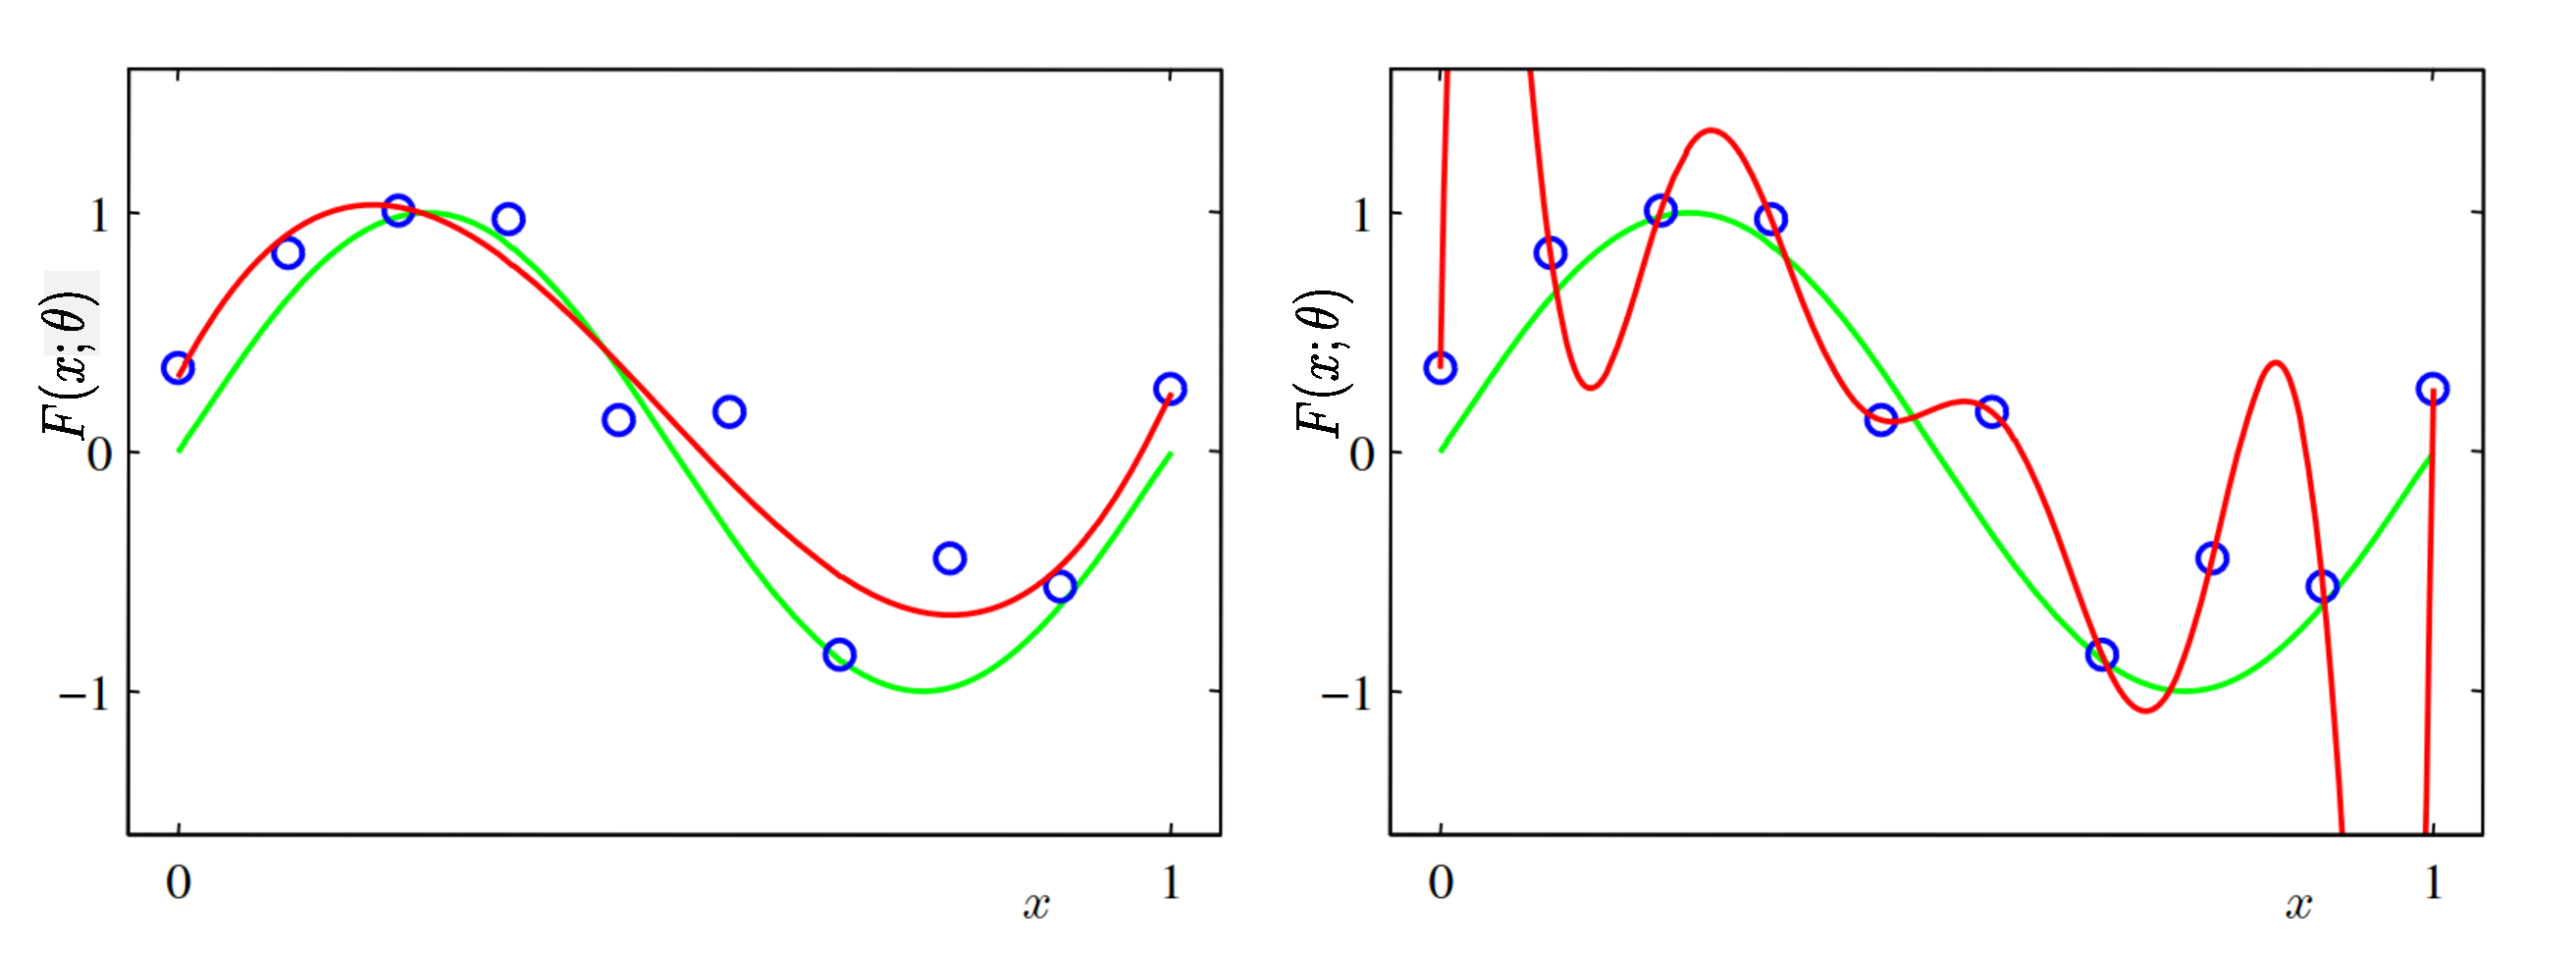
\includegraphics[width=\linewidth]{overfitting.eps}
  \caption{Comparison between model biased to the training data (right) and model
  that achieves bias-variance trade-off (left)~\cite{bishop2006pattern}. Blue
  circles represent training data, the green curve is the original data source
  for which we are learning a regression model, the red line is the learned
  model $F(x;\theta)$}.
  \label{fig:overfit}
\end{figure}

\subsubsection{Posterior Distribution}

While the likelihood and prior distributions in~\eqref{eq:bayes_posterior} can
be expressed explicitly, the evidence $P(\mathbb{D})$ is typically intractable.
We leverage Bayesian inference techniques to approximate or find the exact
posterior distribution without the use of the evidence. Two of the most famous
techniques are discussed as follows.
\begin{enumerate}
  \item \textbf{Markov Chain Monte Carlo (MCMC) methods}: find the exact
  posterior distribution from a collection of samples of $\theta$.
  %
  MCMC methods collect these samples from a proposal distribution
  $\tilde{Q}(\theta^{(\tau)} | \theta^{(\tau-1)})$, where the sequence of
  samples $\theta^\tau$ form a Markov Chain~\cite{bishop2006pattern}.
  %
  The proposal distribution is known up to its normalization constant and is
  sufficiently simple to sample from. 
  %
  We accept or reject each candidate sample according to the following rule~\cite{bishop2006pattern}:
  \begin{align*}
    \nu &\sim \mathbb{U}(0, 1), \\
    A(\theta^{(\tau)}, \theta^{(\tau-1)}) &= \min \Biggl(1, \frac{P(\mathbb{D} | \theta^{(\tau)})P(\theta^{(\tau)})}{P(\mathbb{D} | \theta^{(\tau-1)})P(\theta^{(\tau-1)})} \Biggr),
  \end{align*}
  \noindent where $\mathbb{U}$ is the uniform distribution. If
  $A(\theta^{(\tau)}, \theta^{(\tau-1)}) \geq \nu$, then we accept the sample. 
  %
  Otherwise, we discard the candidate and resample from $\tilde{Q}(\theta^{(\tau)} |
  \theta^{(\tau-1)})$.
  %
  MCMC methods such as Metropolis-Hastings collect the next sample through
  random walk~\cite{gilks1995markov}, while other gradient-based techniques such
  as Hamiltonian Monte Carlo (HMC) method, efficiently search the
  parameter space through the gradient of the likelihood.
  %
  Even though the MCMC methods learn the exact posterior distribution, they have
  slow convergence properties for high-dimensional parameters. In such cases,
  techniques such as variational inference compromise accuracy of the posterior
  distribution for speed of convergence.
  
\item \textbf{Variational Inference (VI)}: is a gradient-based technique that approximates the posterior with the pre-selected
distribution $Q(\theta;z)$.
%
The approximate posterior is selected from the conjugate families of the
likelihood and prior distributions. The goal is to learn the distribution
parameters $z$ of the approximate posterior that minimize the Kullback-Leibler
divergence or equivalently maximize the evidence lower bound
(\textsc{Elbo})~\cite{cohen2016bayesian}. The \textsc{Elbo}, $\mathcal{L}$, is
given by
\begin{align}
  \begin{split}
  \mathcal{L}(\mathbb{D},z) &= \mathbb{E}_{\theta \sim Q} \left[\log(P(\mathbb{D} \mid \theta;z)P(\theta)) - \log(Q(\theta;z)) \right].
  \end{split}
  \label{eq:elbo}
\end{align}
\end{enumerate}

\begin{rem}
  For continuous posterior distribution, the \textsc{Elbo} given in
  equation~\eqref{eq:elbo} is redefined using differential entropy, which
  expresses the prior and posterior in terms of their probability density
  functions. In this case, the likelihood $P(\theta \mid \mathbb{D};z)$ is also
  a probability density function and the \textsc{Elbo} is not bounded by zero.
\end{rem}

% \subsubsection{Prediction}

Once we find the exact or approximate posterior, the prediction for state $x$
can be found in one of two ways. The first option is to marginalize the model
over the posterior as follows~\cite{jospin2020hands}
\begin{equation}
  \hat{F}(x) = \frac{1}{N_{\theta}} \sum_{\theta \sim Q} F(x; \theta),
  \label{eqn:marginalization}
\end{equation} 
where $N_{\theta}$ is the number of samples drawn from the posterior. 
%
% The marginalization technique is key to combating overconfident predictions
% from overfit models~\cite{bishop2006pattern}.
%
% By sampling and marginalizing over several parameters from the posterior, we are
% averaging over an ensemble of predictions.  
%
The second option only takes one sample from the posterior, and it corresponds
to the maximum aposteriori (MAP), i.e. 
\begin{align} 
  \theta_{MAP}=\underset{\theta}{\textrm{argmax}}\; P(\theta | \mathbb{D})
\end{align}

